\subsection{The Sprint cycle}

In our (close to) one month project period we managed to fit in tree one-week Sprints as well as a short preparing \textit{Sprint Zero}, as is sometimes used in Scrum. The Sprint Zero was focused on the discussion of our vision for the product, identifying initial items for the Product Backlog, providing a minimal environment that enables the  writing of quality code, and other preparation we saw fit e.g. group constitution.

Sprint Zero aside, we made use of Scrum specific meetings and progress tracking tools in our Sprints. In this section we will elaborate on the work process with these tools. It should be noted that the meetings and tools mentioned in the following sections are repeated each Sprint.


\subsubsection{Sprint Planning Meetings} 
Our Sprints were prepared by two short meetings of one hour each. The first of the Sprint Planning Meetings was focused on the "what", while the second is focused on the "how".

In \textbf{Sprint Planning Part One}  we discussed our priorizations of items in our Product Backlog. This part of the meeting was heavily influenced by the Product Owner as he was responsible for the Return of Investment. As such this part of the meeting was primarily focused on the Product Owner explaining his thoughts to the Team (and ScrumMaster) regarding what items should be chosen and also \textit{why} that is the case.

In \textbf{Sprint Planning Part Two} we discussed what items from the Product Backlog should be implemented in the current Sprint. An important aspect of this is meeting was that while the Product Owner heavily influences the priority in the Product Backlog, it was the Team that ultimately chose how many of those items to take on in the Sprint (with highest priority items chosen first). This division of work makes the each Sprint more reliable, as the Team knows how much work they can handle. At the end of the Sprint Planning Meetings we placed the chosen items from the Product Backlog into a \textbf{Sprint Backlog} in our Pivotal Tracker online tool. 

\subsubsection{Daily Scrums}
During the Sprints we had regular very short meetings (10-15 minutes) which was focused on the team members updating each other and coordinating work according to the current status on items in the Sprint Backlog. In a work environment this meeting should happen every workday, but due to other courses we had them scheduled for tuesday, thursday and either saturday or sunday. Our Daily Scrums were based on the three points (1) What has been accomplished since the last meeting?; (2) What will be done before the next meeting?; and (3) What obstacles are in the way?

If any any obstacles were present it was our ScrumMaster's job to help resolve them. Any resolving of problems happened \emph{after} the Daily Scrum had finished in order to keep the meeting itself very precise and to the point, as to not waste the whole Team's time.


\subsubsection{Progress Tracking Tools}
An important point in Scrum is that the Team is a self-managing entity. As evident in the distribution of roles there is no project leader involved (the ScrumMaster should \emph{not} be confused with such), and this requires the Team itself to keep track of progress. The already mentioned Daily Scrum is an important part of this, but there is also other tools available.

\paragraph{Item status}
In a work environment Sprint Backlogs are sometimes maintained as stickers on a big board (called a \textbf{Scrum Board}), which provides an easy overview of the current status. This was not possible (or reliable at least) at our university as we can not reserve the white boards or rooms. Fortunately our online tool has several status states for each items, which we made heavy use of (Statuses include Unstarted, Started, Finished, Delivered, Approved, Rejected).
\begin{figure}[htb]
	\centering
	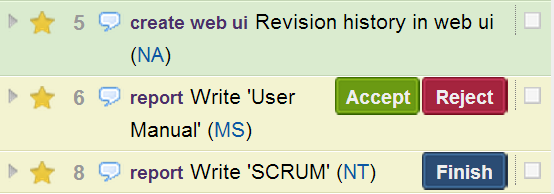
\includegraphics[width=0.75\textwidth]{SCRUM/graphics/status-example.png}
	\caption{An example of statuses on items in the Sprint Backlog}
	\label{fig:item-status}
\end{figure}

\paragraph{Daily estimates}
Another common approach to progress tracking in Scrum is to update the Sprint Backlog with daily estimates of the remaining effort (given in points). In Pivotal Tracker this is done by splitting the big items (an \textit{Epic} in Pivotal Tracker terminology) up into lesser related items (\textit{stories} in Pivotal Tracker terminology).
\begin{figure}[htb]
	\centering
	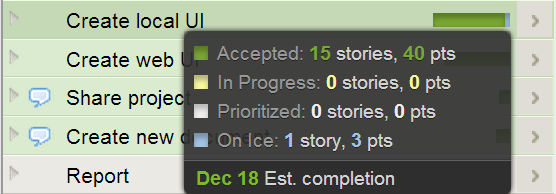
\includegraphics[width=0.75\textwidth]{SCRUM/graphics/epic-example.png}
	\caption{An example of progress tracking on an Epic (Pivotal Tracker terminology)}
	\label{fig:epic-example}
\end{figure}

The last progress tracking tool we've used, which is very common in Scrum-based development, is a  \textbf{Sprint Burndown Chart}. Pivotal Tracker generated this chart (among others) for us, thus making it easy to track how much work was left to be done each Sprint.
\begin{figure}[htb]
	\centering
	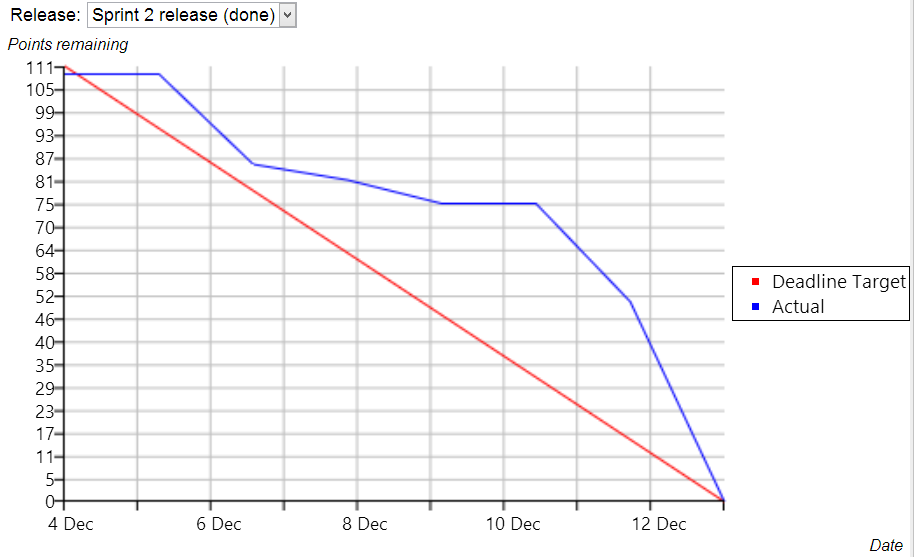
\includegraphics[width=0.75\textwidth]{SCRUM/graphics/burndown-chart.png}
	\caption{Our burndown chart for Sprint 2}
	\label{fig:burndown-chart}
\end{figure}

\subsubsection{Sprint Review}
- Inspection of product

\subsubsection{Sprint Retrospective}
- Inspection of process